% 0236(본책 46쪽) — 평행사변형 ABCD(AB=5, AD=8, ∠ABC=60°), 두 대각선의 교점 O, △AOD·△BOC 색칠. 스캔 삽화를 TikZ 로 다시 그림. 답(넓이)은 적지 않는다.
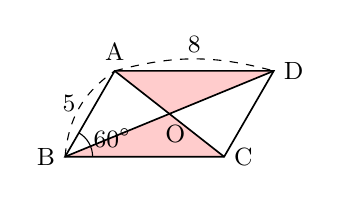
\begin{tikzpicture}[line width=0.6pt]
  \coordinate (A) at (0.63,1.09); \coordinate (B) at (0,0); \coordinate (C) at (2.02,0); \coordinate (D) at (2.65,1.09); \coordinate (O) at (1.325,0.545);
  \fill[red!20] (A) -- (O) -- (D) -- cycle;
  \fill[red!20] (B) -- (O) -- (C) -- cycle;
  \draw (A) -- (B) -- (C) -- (D) -- cycle;
  \draw (A) -- (C);
  \draw (B) -- (D);
  \draw[line width=0.4pt] (0.35,0) arc[start angle=0, end angle=60, radius=0.35];
  \node[font=\small] at (0.6,0.24) {$60^\circ$};
  \draw[dashed, line width=0.4pt] (B) to[bend left=25] (A);
  \node[font=\small] at (0.05,0.68) {$5$};
  \draw[dashed, line width=0.4pt] (A) to[bend left=15] (D);
  \node[font=\small] at (1.64,1.42) {$8$};
  \node[font=\small, above] at (A) {A};
  \node[font=\small, left] at (B) {B};
  \node[font=\small, right] at (C) {C};
  \node[font=\small, right] at (D) {D};
  \node[font=\small, below] at (1.4,0.52) {O};
\end{tikzpicture}
